%!TEX root=thesis.tex
%This is the draft literature review. 

%!TEX ROOT = thesis.tex


\chapter{Background Studies}
\label{section:litreview}

In this chapter, related theoretical background concepts are first introduced. Then, the related works are discussed in two main portions: 
\begin{enumerate}
    \item Existing methodology and techniques used for semantics extraction
    \item Recent methodology and techniques used for semantic retrieval.
\end{enumerate}



\section{Related Theoretical Background Concepts}
\label{subsec:relatedConcepts}

Before diving deeper into the nitty-gritty of the proposed framework, fundamental understanding towards related theoretical background concepts used in this work is discussed. As this work covers a rather broad spectrum of different concepts, a general understanding towards these concepts would provide some degree of clarity towards the topic at hand. This section briefly describes the fundamental of the following concepts: i) Quantization, ii) Distance Measure, iii) Human Visual System, \& iv) colour Model and colour Terms. 


\subsection{Quantization}

The use of quantization in the mathematical and digital signal processing field is not a new concept. Digital signal processors are limited by natural boundaries such as hardware limitations, and are only able to compute and perform arithmetic operations within a limited range \cite{spors_2018}. The use of quantization refers to the process of mapping and projecting a set of large values which are often continuous or analog in nature into a set of discrete and finite values. 

\begin{figure}[hbt!]\centering
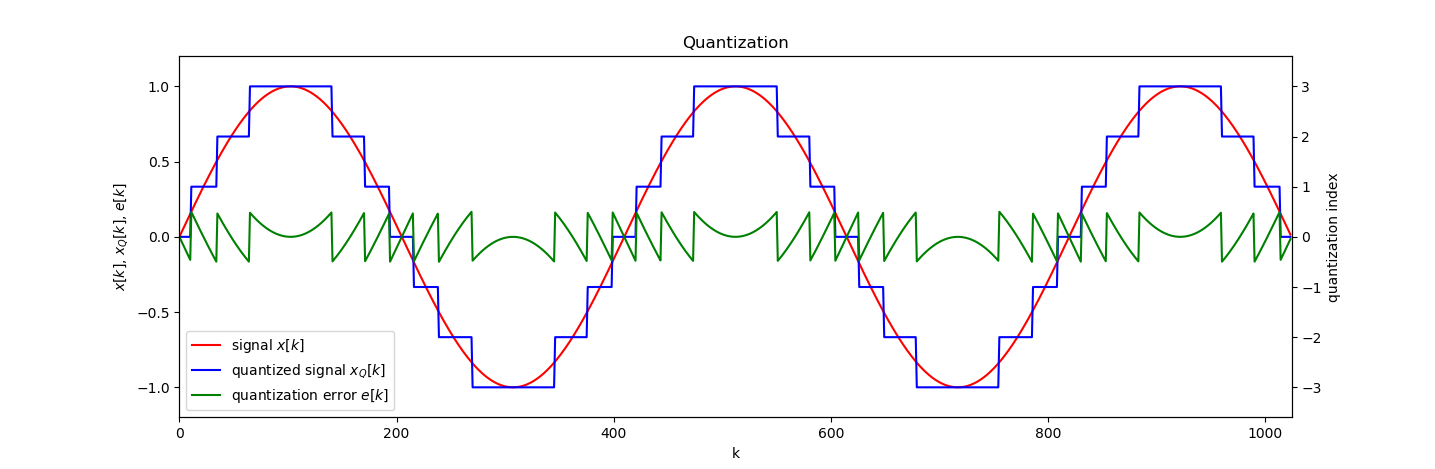
\includegraphics[width=\textwidth]{image/general/quantization.png}
\caption{Quantization}
\label{fig:quantize}
\end{figure}


The use of quantization enables reduction in memory usage (compression) as well as the reduction of computational cost, hence, leading to faster processing speed. However, since the quantization process is a many-to-few mapping operation, the operation is considered irreversible without prior knowledge of the loss. Nevertheless, the output discrete signal can closely resemble the continuous input signal depending on the number of quantization level used.
\begin{equation}\centering
\label{eq:quantization}
x_Q[k] = g( \mspace{3mu}\lfloor \mspace{3mu}f(x[k]) \mspace{3mu}\rfloor\mspace{3mu})
\end{equation} 
\vspace{-3em}
\begin{equation}\centering
\label{eq:quantizationerror}
e[k] = x_Q[k] - x[k]
\end{equation}
In order to expound on the quantization process, a mathematical model of this process can be formulated as such. Consider a continuous signal $x[k]$ whose quantized signal, $x_Q[k]$, is desired (see Equation \ref{eq:quantization}). The functions $f (\mspace{3mu} \cdot  \mspace{3mu})$ \& $g (\mspace{3mu} \cdot  \mspace{3mu})$ can be thought of as a real-value mapping function while the $\lfloor \mspace{3mu} \cdot  \mspace{3mu} \rfloor$ represents a rounding function. The $f (\mspace{3mu} \cdot  \mspace{3mu})$ function is used to convert real-world values into a digital signal, while $g (\mspace{3mu} \cdot  \mspace{3mu})$ is used to map the digital signal into a quantized signal. As previously mention, this process is considered irreversible with prior knowledge of the loss, in this case, the quantization error, $e[k]$, can be computed as Equation \ref{eq:quantizationerror}. Figure \ref{fig:quantize} illustrates a quantization process where the red signal ($x[k]$) represents the real-world continuous signal, the blue signal ($x_Q[k]$) refers to the quantized signal while the green signal ($e[k]$) represents the error due to quantization process.

In order to leverage on this concept, in this work, the quantization technique was extended further into a three dimensional space. As video data can be represented in a 3D space, the quantization process was used to quantize the continuous video data into a set of discrete and finite values. These discrete and finite values can ease the calculation and manipulation of data. As colour space can also be represented using a 3D space, this concept was adapted and applied here to quantize the colour space into colour terms (See Section \ref{section:colourterm}).



\subsection{Distance Measure}
\label{section:distancemeasures}

The use of distance measure is another recurring key concept in the proposed method. Given that distance measures are commonly used in computer science as well as the mathematics field, there are numerous metrics suggested by different authors which are applicable and useful in different scenarios. In essence, distance measure is used to compute the difference between targets. On the flip side, the difference can also be thought of as the similarity between these targets.

\begin{figure}[hbt!]\centering
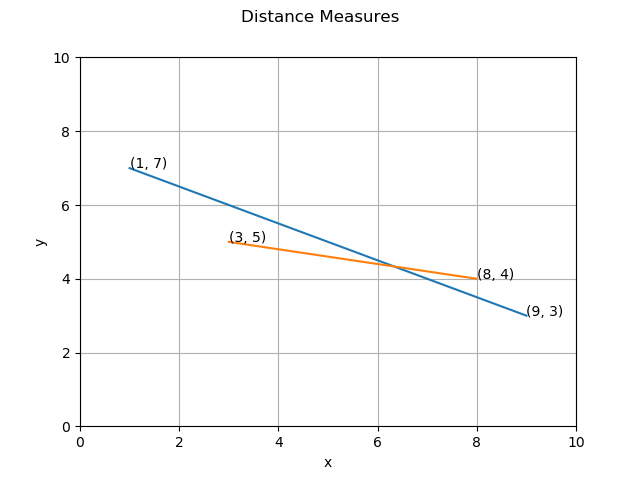
\includegraphics[width=.7\textwidth]{image/general/distance.png}
\caption{Example of Distance Measure}
\label{fig:distanceMeasure}
\end{figure}

To further accentuate on the concept of distance measure in this work, a simple example of how distance metrics can be applied in the proposed method is illustrated using Figure \ref{fig:distanceMeasure} with two plotted lines. In order to simplify the research problem, these lines can be thought of as vehicle trajectories captured over time that is flatten unto a 2D plot. Using the available data, the distance between two trajectories can be measured and used to signify the dissimilarity between them. This distance measure can also be used to identify trajectories with high resemblance. 

\begin{figure}[hbt!]\centering
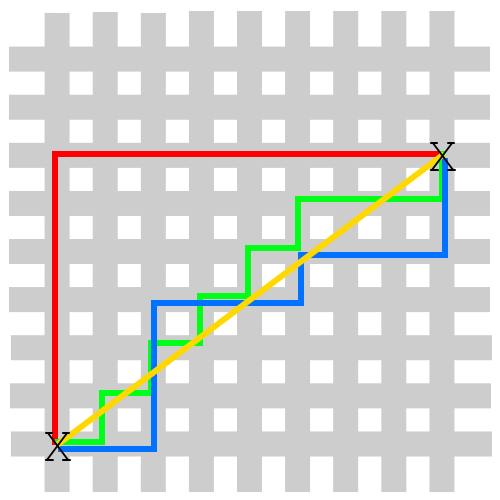
\includegraphics[width=.5\textwidth]{image/lit/manhattan.png}
\caption[Comparison between Manhattan Distance vs. Euclidean Distance]{With the assumption that each block has a equal distance of 1. Using Manhattan Distance, regardless of the path taken, the distance for the red, green and blue lines has the length of $14$. These 3 paths, while different, still takes on the shortest distance from one end to the other. However, when computing using Euclidean Distance, the distance is measured to be $\sqrt{8^2+6^2} = 10$. Euclidean Distance only produces $1$ unique solution while Manhattan Distance may produce more than one solution.}
\label{fig:manhattan}
\end{figure}


However, as different distance measure metrics are suitable for different scenarios, a good distance measure is an essential for comparing a significantly extensive set of vehicle trajectories during the retrieval process of a car park scene. This concept of distance measure was further extended into a multi-dimensional space such as the colours space, where the similarity between two or more colours were measured using different distance metrics to evaluate the performance of each metric. Table \ref{table:distance} lists out several distance measure which are commonly used along with the pros and cons of each while Figure \ref{fig:manhattan} shows the contrast between Euclidean and Manhattan distance.

\begin{table}[!ht]
\resizebox{\textwidth}{!}{
\begin{tabular}{|l|l|l|}
\hline
\textbf{Distance Measure} & \textbf{Pros} & \textbf{Cons} \\ \hline
Euclidean Distance & \begin{tabular}[c]{@{}l@{}}Simple, Fast,\\ Commonly used,\\ Able to work on n-Dimension data\end{tabular} & \begin{tabular}[c]{@{}l@{}}Vector order dependent,\\ Requires same length vectors\end{tabular} \\ \hline
Manhattan Distance & \begin{tabular}[c]{@{}l@{}}Reflection invariant,\\ Translation invariant,\\ Produces same result,\\ Able to work on n-Dimension data\end{tabular} & \begin{tabular}[c]{@{}l@{}}Requires same length vectors,\\ Does not have a unique solution\end{tabular} \\ \hline
Chamfer Distance & \begin{tabular}[c]{@{}l@{}}Able to work with \\ vectors of different length,\\ Vector order invariant, \\ Minimizes the difference \\ between vectors,\\ Able to work on n-Dimension data\end{tabular} & \begin{tabular}[c]{@{}l@{}}Higher computational cost,\\ Alternative matches may \\ receive equal distance\end{tabular} \\ \hline
Hamming Distance & \begin{tabular}[c]{@{}l@{}}Ensure similarity between vectors,\\ Able to work on n-Dimension data\end{tabular} & \begin{tabular}[c]{@{}l@{}}Vector order dependent,\\ Requires same length vectors\end{tabular} \\ \hline
\end{tabular}%
}
\caption{List of several distance measures along with their pros and cons}
\label{table:distance}
\end{table}




\subsection{Human Visual System}
\label{section:eyes}
The human eyes are visual system organs, responsible of receiving and processing visual information. Figure \ref{fig:eyes} shows a rough anatomy of the human eye. Within the eye, rods and cones are light-sensitive cells, found on the retina which are in charge of vision. Both of these cells plays a different role, rods cells are not able to perceive colour information, hence, they are known to be responsible for determining the lighting condition. On the other hand, cones cells are responsible for the reception of colour information. As human retina contains approximately 120 million rods and 6 million cones, the eyes are more sensitive toward lighting conditions. The sheer number of rods also enables humans to see in low-light achromatic vision.   


\begin{figure}[hbt!]\centering
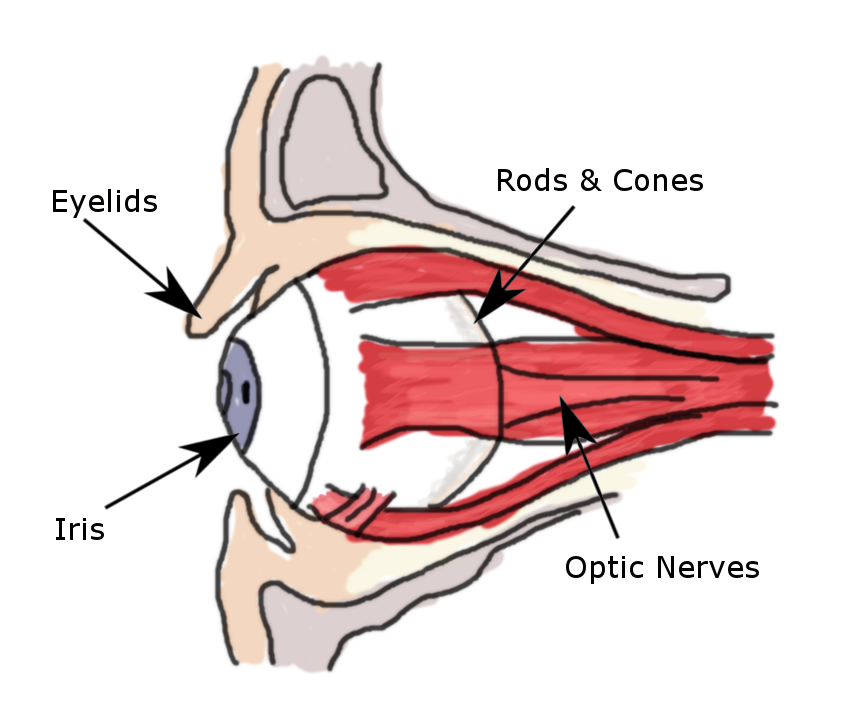
\includegraphics[width=.5\textwidth]{image/lit/rodsandconscolored.png}
\caption[Human Eye Anatomy]{Human Eye Anatomy. Rods and cones cells are responsible over human vision. When these cells on the retina are stimulated, signals are sent to the brain via the optic nerves. The brain would then processes these signals to provide vision for humans.}
\label{fig:eyes}
\end{figure}

Anatomically, there are three types of cones in the human retina, each of which are responsible over the receptiveness of colours in a particular type of wavelength. These wavelengths can be classified into three main categories: Short wavelengths light, Medium  wavelengths light and Long wavelengths light (See Figure \ref{fig:visibleSpectrum} \cite{eyespectrum}). colours are perceived from the combination of stimuli to these rods and cones cells and responses from brain. When stimulated, these cells fires electrical signals to the optic nerves fibres that communicates with the brain. However, as the number of cones cells in the retina varies for each person, the colour perception of everyone would differ in a way or another. 


\begin{figure}[hbt!]\centering
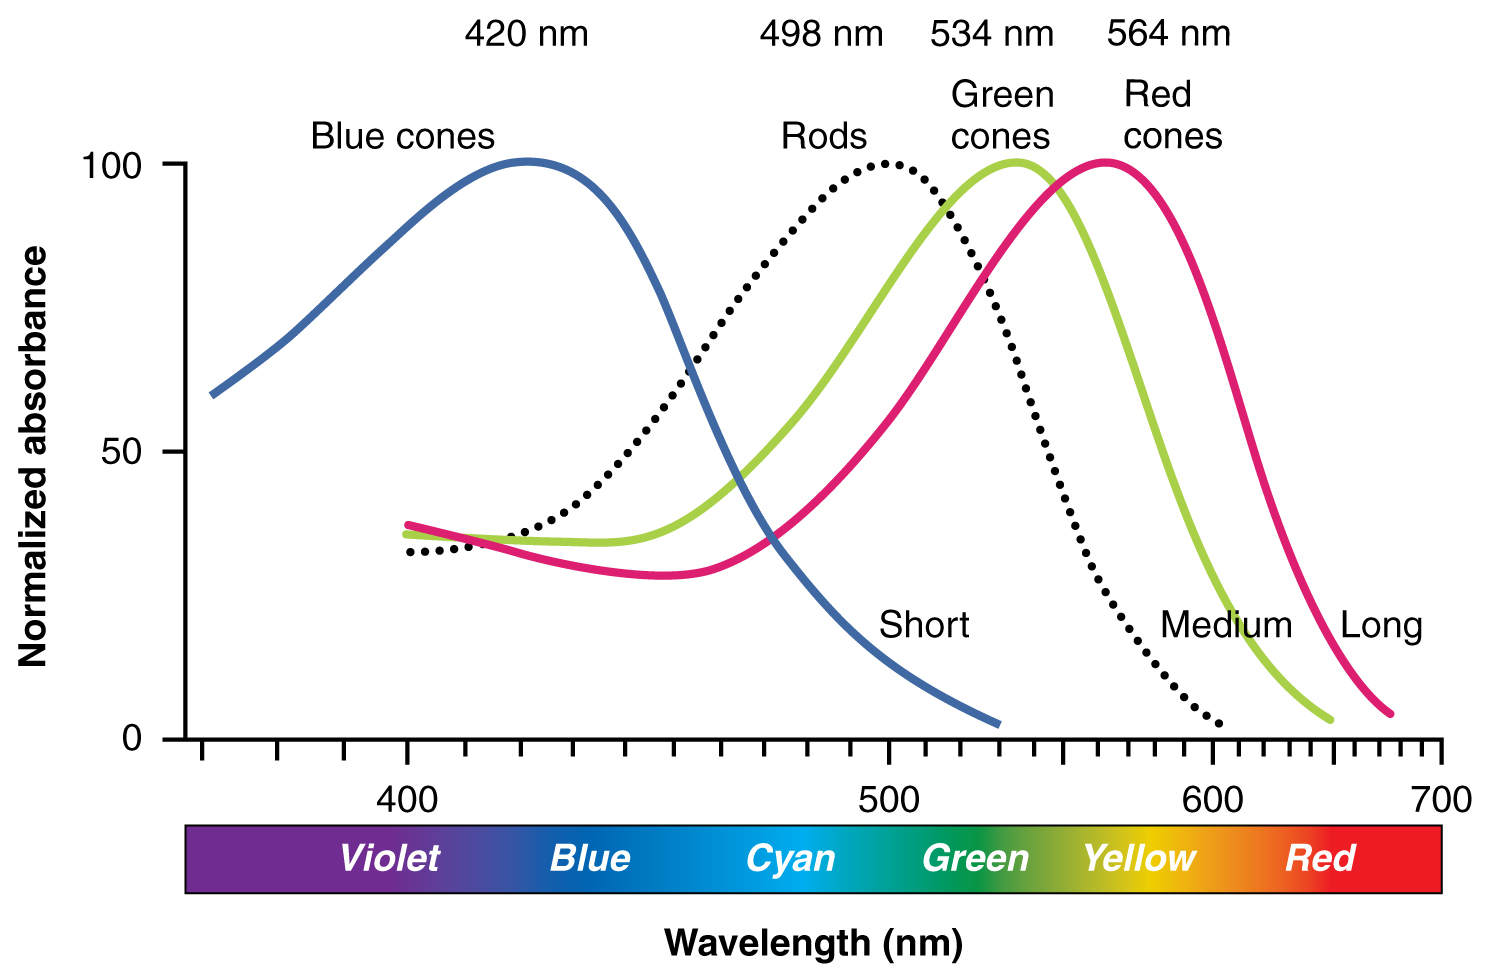
\includegraphics[width=.7\textwidth]{image/lit/ColorSensitivity.jpg}
\caption[Normalised human photo-receptor absorbency rate for different wavelength lights]{Normalised human photo-receptor (cons \& rods) absorbency rate for different wavelengths of light. 'Blue' cones, approximately 420-440 nm, are short wavelengths light; 'Green' cones, approximately 534-545 nm, are medium wavelengths light; and, 'Red' cones, approximately 564-580 nm, are long wavelength lights }
\label{fig:visibleSpectrum}
\end{figure}




\subsection{Colour Model, Systems and Terms}
\label{section:colourterm}

In order to represent colours in tuples of number, colour models were designed. In essence, it can be thought of a quantization process of converting a series of real-world continuous signal (colour wavelengths) into a set of finite tuples of numbers within a colour model. 
With the ability to quantize these wavelengths into sets of finite tuples, the colours can be digitised and used for further processing.


\subsubsection{Colour Models}
From the previous section, the humans' visual system was explored. From there, it is learnt that the cones cells in the retina are strongly receptive towards stimuli of 'Red', 'Green' and 'Blue' wavelengths. Given the solid theory behind human perception of colours, the RGB colour model was designed. This colour model is commonly used to represent and display images in digital systems. 

As an example, the RGB colour space is an additive colour model, each of the components (R, G, B) are added together to produce the final colour. Typically each of these components are represented using 8 bits, hence, 256 possibilities for each component with a total of $256 \times 256 \times 256 = 16M$ colour combinations in total. As this is an additive model, 'Black' colour is  represented using $(0, 0, 0)$, while 'White' using $(255, 255, 255)$. Figure \ref{fig:rgb} represents this colour model.

\begin{figure}[hbt!]\centering
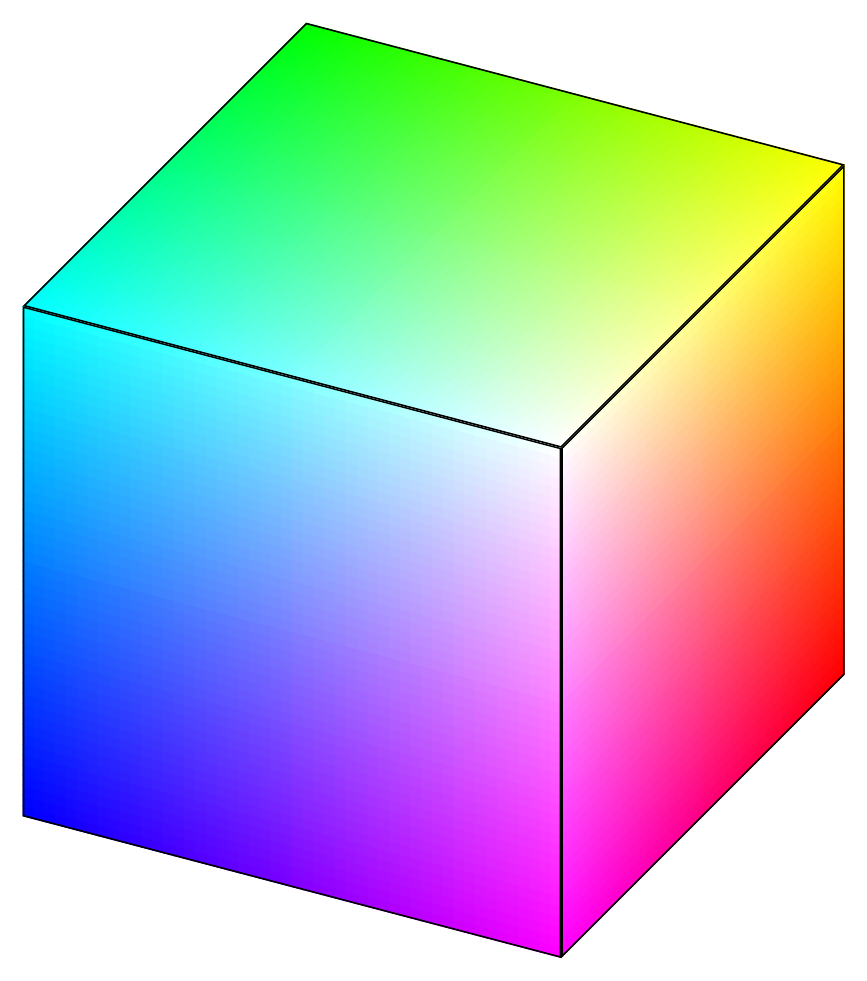
\includegraphics[width=.4\textwidth]{image/lit/rgbcolor.jpg}
\caption{RGB colour Model}
\label{fig:rgb}
\end{figure}


\subsubsection{Munsell Colour System}
\label{section:munsellcs}
colour terms - such as "Red", "Green" or "Blue", are commonly derived from the Munsell colour system which was created in the early 20th century by Professor Albert H. Munsell. The Munsell colour System was designed to organise colours similar to how the human's eye sees - which is, by organising colours according to their hues, followed by the chromatic range and the brightness values in a perceptually uniform manner. 

For each horizontal circle on the Munsell colour System, the hues can be divided into 5 principle hues which are Red, Yellow, Green, Blue, and Purple. This setup allows another 5 intermediate hues in between each principle hues, for example: Green-Blue hue, Purple-Red hue. 
Figure \ref{fig:munsell}(a) illustrates the Munsell colour System while Figure \ref{fig:munsell}(b) illustrates the property of the chroma and value scale available on the Munsell colour system, for example, a hue at 2.5 Yellow-Red (YR) has a maximum chroma value which differs along the value axis. 



\begin{figure}[!htb]
  \centering
  \resizebox{\textwidth}{!}{
\begin{tabular}{cc}
 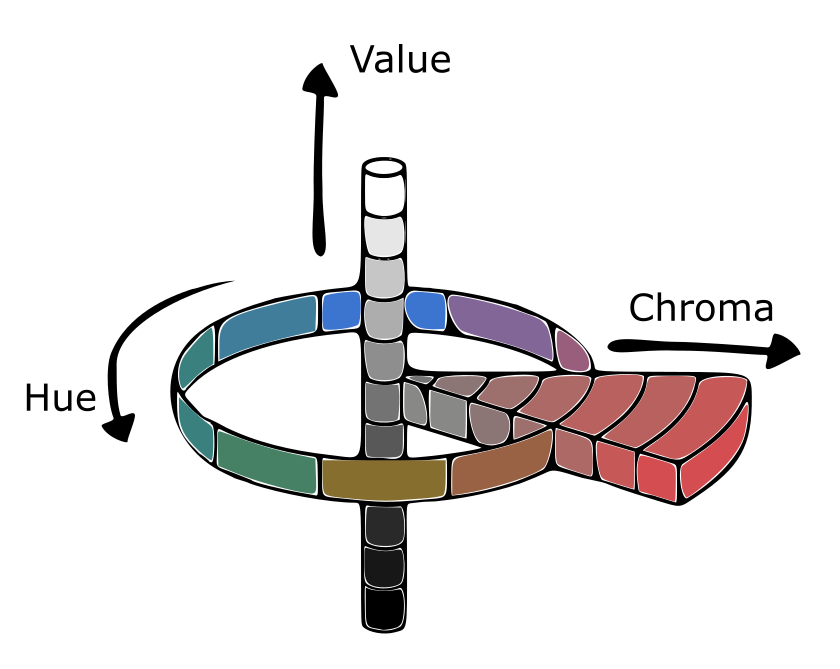
\includegraphics[width=0.4\linewidth]{image/general/munsell.png}  &
 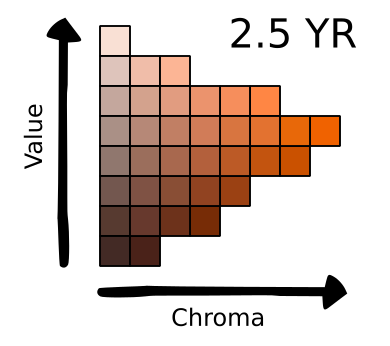
\includegraphics[width=0.4\linewidth]{image/general/25YR.png}\\
 (a) Munsell colour System &
(b) Hue at 2.5YR with various Chroma and Value\\
\end{tabular}}
\caption{Munsell colour System} \label{fig:munsell}
\end{figure}



\subsubsection{Colour Terms}

While the basic idea of colours seems to be a relatively simple idea for humans, machines on the other hand, do not understand the concept of colours. Modern computers generally represents colour values using the Red-Green-Blue (RGB) values for most applications. Despite its frequent usage, it is difficult for humans to visualise a particular colour when presented with three RGB values as these values does not directly translate the intuitive nature of a particular colour. Along with that, it is also very difficult to visualise the difference between two colours using the RGB values only. 

Table \ref{table:allcolourterms} lists several popular web colour dictionaries along with the number of colour terms as well as the publishing year. One notable property of these colour terms is the use of compound terms such as 'baby blue', 'dark red', 'light purple' and 'very deep brown'. Along with that, in some colour dictionary, certain colours terms are duplicated for several tuples. Given the variety of colour dictionaries and the number of different colour terms, one of the targets in this work is to investigate and decide how many colour terms should be allocated to describe the vehicle colours. 

\begin{table}[hbt!]
\centering
\begin{tabular}{|c|c|c|}
\hline
\multicolumn{1}{|c|}{\textbf{Web Colour Dictionary}} & \multicolumn{1}{c|}{\textbf{Number of Colour Terms}} & \multicolumn{1}{c|}{\textbf{Year}} \\ \hline
x11 (R3)                                            & 631                                                 & 1988                               \\ \hline
HTML                                                & 140                                                 & Current                            \\ \hline
CSS                                                 & 148                                                 & Current                            \\ \hline
Crayola                                             & 248                                                 & Current                            \\ \hline
xkcd                                                & 954                                                 & 2010                               \\ \hline
\end{tabular}
\caption[Web Colour Dictionary and the corresponding number of colour terms]{Web Colour Dictionary and the corresponding number of colour terms}
\label{table:allcolourterms}
\end{table}

%https://people.csail.mit.edu/jaffer/colour/Dictionaries
% x11 colours: https://groups.google.com/forum/?fromgroups=#!topic/comp.windows.x/AYPozZhQxok
% https://www.crayola.com/explore-colours.aspx
%http://markkness.net/colourpy/colourPy.html



In a classic study of worldwide colour naming, \citeA{berlinandkay} proposed that the naming of colours terms may differ due to different cultures. Based on their findings, native English language speakers generally used eleven basic colour terms. These terms had to have three common properties which are: i) Highly used, ii) Monolexemic - meaning a single(mono) word, and not compounded colour term such as 'baby blue', and iii) agreed upon by native speakers of the language. With those definitions, the common colour terms proposed for the English language are black, white, gray, brown, red, orange, yellow, purple, green, blue, and pink. The 11 common colour terms were also adopted by several other authors (\citeA{van2009learning}, \citeA{zaslavsky2018efficient}, and \citeA{yu2018beyond}) in their work to understand how these colour terms can be used for real-world image applications. However, \citeA{yu2018beyond} also remarked that most existing work on colour names focuses on only the eleven basic colour terms of the English language, however, this could be limiting the discriminative power of these representations. 







\section{Related Works}
\label{section:relatedworks}

The advancement of computer vision technologies enabled the development and integration of various solutions to tackle challenges in Intelligent Transportation Systems (ITS). As ITS is a big topic, there has been a substantial increase of research done on the various subdomains. With the amount of research done, instead of reinventing the wheel, existing frameworks were adopted and leveraged upon. Recent survey done by \citeA{tian2017hierarchical} and \citeA{chandran2017review} were studied to understand the general overview of the state of related works. The authors has summarised the challenges that are often found in an ITS setting that is implemented on a one-camera setup: 
\begin{enumerate}
    \item \textbf{Camera placement} affects the overall performance. 
    \item The \textbf{lighting condition} varies throughout the day. Supplemental lighting equipment can be used during the night, however, the visual range will be limited.
    \item Vehicles are often \textbf{occluded} in an ITS setting; often by pedestrians, bicycles, trees, and even buildings.
    \item \textbf{Vehicle pose} varies when turning or changing lanes.
    \item Vehicles comes in a \textbf{variety of shapes, sizes, and colour.}
    \item As \textbf{vehicles' size changes} as it pass through the camera's field of view. This variation in visual information affects the robustness of some detection models. 
\end{enumerate}
Along with that, \citeA{tian2017hierarchical} presented an overview of the general frameworks for ITSs with the aim of vehicle attribute extraction and behaviour understanding in Figure \ref{fig:ITSoverview}. According to \citeA{liu2016deep}, in a real-world scenario, appearance features such as colours, shapes, and types are very effective to filter out the dissimilar vehicles. In addition, they are efficient to be extracted and searched in large-scale dataset. 
As mentioned in Section \ref{subsec:scope}, the bounding box of each vehicles are assumed to be obtained prior to the semantic extraction task, related literature regarding the detection and tracking of vehicles will not be discussed. 
Instead, the rest of this section is expounded under two main categories: i) Objects Semantic Extraction, and ii) Object Semantic Retrieval. 


\begin{figure}[hbt!]\centering
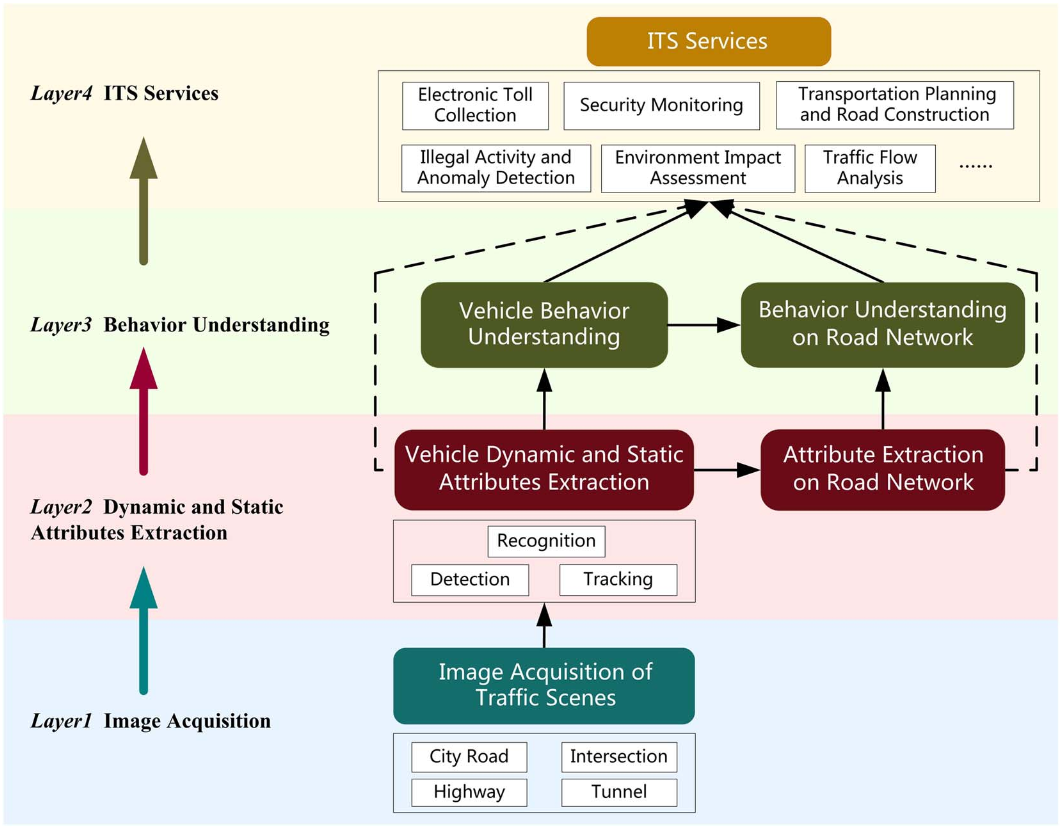
\includegraphics[width=1\textwidth]{image/lit/ITS.png}
\caption[Overview of the General Frameworks for ITSs]{(From Bottom) Layer 1: The process of obtaining data via vision sensors. Layer 2: Attribute Extraction from data; this includes motion, trajectories, colours, shapes and etc. Layer 3: Analysis on vehicle behaviours from the extracted attributes to decide traffic status. Layer 4: Utilises information from Layer 3 to optimise various ITS services. Figure reproduced from~\citeA{tian2017hierarchical}}
\label{fig:ITSoverview}
\end{figure}




\subsection{Object Semantics Extraction}

\subsubsection{Vehicle Colours Extraction}
The extraction of Vehicle colours is essential for a wide variety of applications in ITS such as crime prevention and security purposes. 
According to \citeA{zhang2017vehicle}, colour is one of the most stable attributes of vehicles and often used as a valuable cue in some important applications.
\citeA{hsieh2015vehicle}, \citeA{chen2014vehicle} and \citeA{zhang2017vehicle} noted that in a surveillance scenario, the varying illumination, coupled with complex environment factors (weather, noise) as well as the camera viewpoint in an outdoor scene affected the classification of colours drastically. 
Various vehicle colour extraction methods has been proposed in the recent years, these methods can be broadly divided into two main categories: i) Hand Crafted Features, and ii) Machine Learned Features.
In \citeA{hsieh2015vehicle}'s work, the vehicles are grouped into seven categories (Figure \ref{fig:sevenclasses}). Given that the source footages were taken outdoor with varying illumination settings, a global colour correction method (Figure \ref{fig:colorcorrection}) was employed to suit different lighting needs. 

\begin{figure}[hbt!]\centering
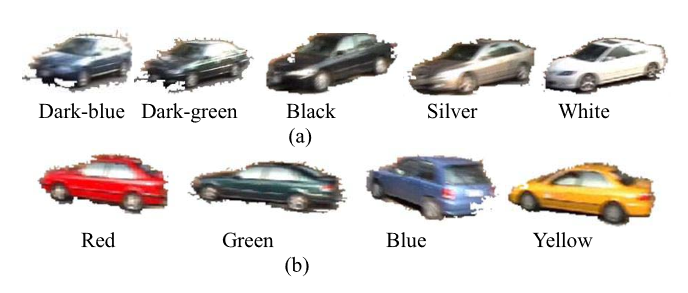
\includegraphics[width=.8\textwidth]{image/lit/carscolors.png}
\caption[Colour Appearance Categories of  Vehicle  Used  for  Colour Classification]{(a) Vehicles Classified as "Achromatic"; (b) Chromatic Vehicles. Reproduced from \citeA{hsieh2015vehicle}.}
\label{fig:sevenclasses}
\end{figure}

\begin{figure}[!htb]
  \centering
 \resizebox{\textwidth}{!}{
\begin{tabular}{ccc}
 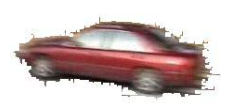
\includegraphics[width=0.4\linewidth]{image/lit/windowremove1.png}  &
 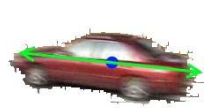
\includegraphics[width=0.4\linewidth]{image/lit/windowremove2.png} & 
 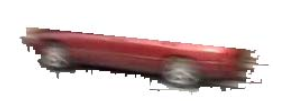
\includegraphics[width=0.4\linewidth]{image/lit/windowremove3.png} \\
 (a) Input Vehicle &
(b) Proposed Cutting Line for Window Removal &
(c) Result of Window Removal\\
\end{tabular}
}
\caption[Window Removal Task. From left: Input Vehicle, Proposed Cutting Line, Results of Window Removal]{Window Removal Task. From left: Input Vehicle, Proposed Cutting Line, Results of Window Removal. Image reproduced from \citeA{hsieh2015vehicle} \label{fig:windowremoval}}
\end{figure}

\begin{figure}[!htb]
  \centering
  \resizebox{\textwidth}{!}{
\begin{tabular}{cccc}
 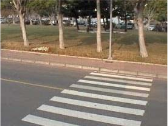
\includegraphics[width=0.3\linewidth]{image/lit/cc1.png}  &
 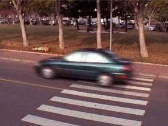
\includegraphics[width=0.3\linewidth]{image/lit/cc2.png} & 
 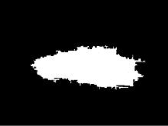
\includegraphics[width=0.3\linewidth]{image/lit/cc4.png} & 
 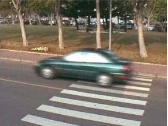
\includegraphics[width=0.3\linewidth]{image/lit/cc3.png} \\
 (a) Reference Image &
(b) Colour Distortion &
(c) Background of (b) &
(d) Result of Colour Correction\\
\end{tabular}
}
\caption[Colour Correction. From left: Reference Image, Image with Colour Distortion, Background of (b), Results of Colour Correction]{Colour Correction. From left: Reference Image, Image with Colour Distortion, Background of (b), Results of Colour Correction. Image reproduced from \citeA{hsieh2015vehicle} \label{fig:colorcorrection}}
\end{figure}

Along with that, occasionally the vehicle windows appear white due to the effects of specular highlights, the authors also proposed a window-removal task to increase the accuracy (Figure \ref{fig:windowremoval}). This work also proposed the classification of vehicles into chromatic and achromatic classes, the final colour category is decided via Support Vector Machine (SVM). The accuracy of differentiating between chromatic and achromatic classes over 10,000 vehicles were reported to be approximately 88\%. \citeA{chen2014vehicle} also suggested a similar approach by implicitly selecting a Region-of-Interest (ROI) to improve the classification performance for both images and video data. These collected data were captured using high-definition cameras with resolutions of $1920 \times 1080$ pixels. In this work, the ROI in the image was selected by assigning different weights which are learnt by a classifier for each of the proposed subregions. 

\citeA{jeong2017homogeneity} took on a different approach in order to extract the vehicle colours by implementing a Homogeneity Patch Search Method. In their work, a voting system as implemented to vote on the dominant colour based on the HSV histograms which were extracted from each patch using Adaboost Classifier. First, the edges from the input image was detected using Sobel edge operators. Next, Distance Transformation was performed using Felzen-szwlb algorithm to obtain the minimal distance to the edges of each pixel. As edges often introduce distortion of colour, this step allows the proposed method to select patches that further from the edges. Figure \ref{fig:colorpatches} illustrates this process. While \citeA{jeong2017homogeneity}'s proposed method obtained an accuracy of 92\% over 7 classes, it was only tested against 208 images that have a relatively high resolution of $1624 \times 1224$ pixels.

\begin{figure}[!htb]
  \centering
  %\resizebox{\textwidth}{!}{
\begin{tabular}{cc}
 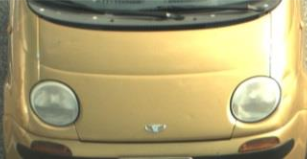
\includegraphics[width=0.3\linewidth]{image/lit/homo1.png}  &
 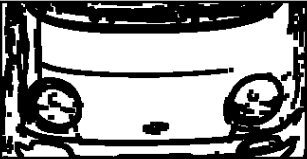
\includegraphics[width=0.3\linewidth]{image/lit/homo3.png} \\
(a) ROI Image &
(b) Inverse of Edge Image \\
 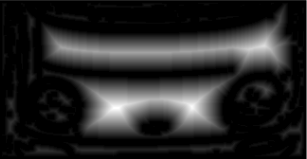
\includegraphics[width=0.3\linewidth]{image/lit/homo2.png} & 
 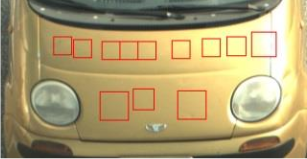
\includegraphics[width=0.3\linewidth]{image/lit/homo4.png} \\
(c) Distance Transformation &
(d) Selected Patches\\
\end{tabular}
%}
\caption[Homogeneity Patch Search from Input. (a) Region of Interest, (b) Inverse of Edge Image Using Sobel Operators, (c) Distance Transformation Calculated using Felzen-szwlb algorithm, (d) Selected Patches Based on Obtained Distance.]{Homogeneity Patch Search from Input. (a) Region of Interest, (b) Inverse of Edge Image Using Sobel Operators, (c) Distance Transformation Calculated using Felzen-szwlb algorithm, (d) Selected Patches Based on Obtained Distance. Image reproduced from \citeA{jeong2017homogeneity} \label{fig:colorpatches}}
\end{figure}

As colour histograms are one of the most common feature used for colour classification task, \citeA{kim2008deciding} aimed to understand the correlation of the number of colour histogram bins used and how different configurations would affect the performance of matching the histogram bins to colour terms using distance measures. This use of histogram bins effectively reduces the processing time needed while promoting recognition accuracy \cite{zhang2017vehicle}. The Hue-Saturation-Intensity (HSI) colour space was used with a total of 17 varying configurations of histogram bins (e.g. 16 bins for Hues, 4 bins for Saturation and 4 bins for Intensity) for the experiment. The results from the experiment shows an average score of 84\%; the best configuration of (H:8, S:4, I:4) achieved an accuracy of 87.83\% over seven colour classes with 100 images per class. 

\citeA{zhang2017vehicle} and \citeA{hu2015vehicle} approached this challenge of extracting colour term by implementing a convolutional neural network (CNN) to extract deep features which are then fed into a linear SVM for the classification task. \citeA{zhang2017vehicle} mentioned that the state-of-the-arts methods takes the whole image for colour recognition, however many parts of the images such as car windows, wheels, and background contributes negatively to the recognition accuracy. A noise reduction method via saliency detection was proposed in order to boost the performance. While this method achieved an accuracy of 94\%, the proposed pipeline with saliency detection, deep feature extraction, dual-orientational dimensionality reduction and classifier training is not suitable for real-time applications.

\begin{figure}[!htb]
  \centering
  %\resizebox{\textwidth}{!}{
\begin{tabular}{cc}
 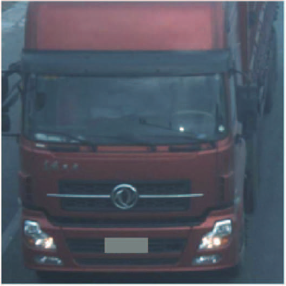
\includegraphics[width=0.4\linewidth]{image/lit/hu1.png}  &
 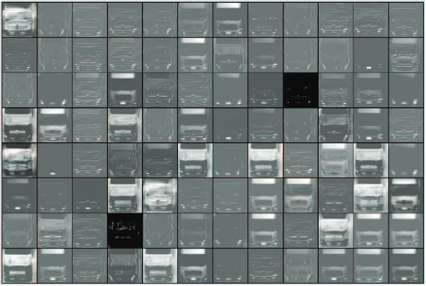
\includegraphics[width=0.6\linewidth]{image/lit/hu2.png} \\
(a) Input Image &
(b) Response Map of the First Convolutional Layer \\
\end{tabular}
%}
\caption[(a) Input and (b) Response from First Convolutional Layer. ]{(a) Input and (b) Response from First Convolutional Layer. Image reproduced from \citeA{hu2015vehicle} \label{fig:responseFCL}}
\end{figure}

According to \citeA{hu2015vehicle}, there are two reason of choosing SVM over fully-connected layers (FCL). The first reason is the ability of SVMs to perform better due to the regularisation contraints that helps overcome overfitting of training data. Another reason why SVM was chosen was due to the fact that SVMs has lesser parameters, this makes the fine tuning process easier. 
Figure \ref{fig:responseFCL} illustrates the input image and the response produced by the first convolutional layer produced in \citeA{hu2015vehicle}'s work. The author claims that the proposed method has advantages over hand-crafted methods that performs the segmentation of subregions, this is because the response map from the first convolutional layer contains meaningful ROIs which are effective for distinguishing vehicle colours. This work achieved an average precision of 93\%, with input data of $1920 \times 1080$ resolution.  
As a whole, while both hand crafted features and machine learnt features methods were able to achieve an accuracy of over 84\%, most of the proposed solutions worked on high resolution data.   

\begin{figure}[hbt!]\centering
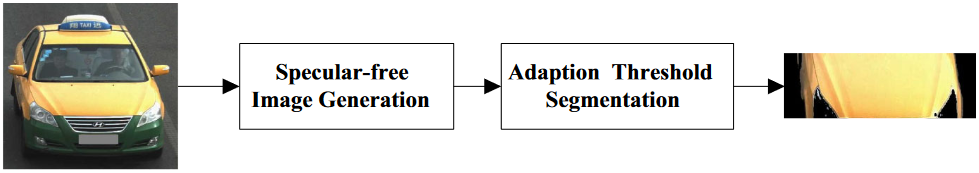
\includegraphics[width=1\textwidth]{image/lit/salient1.png}
\caption[Vehicle-Colour Saliency Detection]{Vehicle-Colour Saliency Detection. Reproduced from \citeA{zhang2017vehicle}.}
\label{fig:Colorsaliency}
\end{figure}

In a semi-related research area of vehicle re-identification, several authors ( \citeA{liu2016deep}, \citeA{liu2016deep2} and \citeA{shen2017learning}) made use of extracted colour features to assist with the re-identification process. \citeA{liu2016deep} adopted the Probabilistic Latent Semantic Analysis (PLSA) introduced by \citeA{van2009learning} to extract the colour features. A PLSA model is used to learn the relation between words (colour terms) and images by providing a conditional probability score. Similar to the work of \citeA{kim2008deciding}, the images in this work were segmented and represented using L*a*b colour histogram of $10 \times 20 \times 20$ grids. \citeA{liu2016deep2} applied deep learning techniques inspired by a triplet loss network proposed by \citeA{ding2015deep}, the network used a new loss function to accelerate the training convergence. The colour features were extracted using the proposed network. Similarly, \citeA{shen2017learning} applied a deep learning network to extract the colour features using a Siamese Network with a shared ResNet-50 configuration. The visual features, including colours, were obtained using the features from the global pooling layers.

\subsubsection{Colour to Colour Term Mapping}

Colour terms are very useful in a real-world application instead of colour tuples. According to \cite{van2009learning}, colour names are required for image retrieval and image annotation applications. 
Several authors has looked into mapping colour tuples into their respective colour terms. \citeA{van2009learning} proposed several variants of Probabilistic Latent Semantic Analysis (PLSA) model to learn colour names from data obtained Google Images. 
This was done in order to avoid hand-labelling real-world images with colour names, Figure \ref{fig:van20091}. The authors approach this challenge by comparing their methods against 3 chip-based methods. 
In their work, chip-based methods was described as colour naming method that is performed in a controlled environment where the labels of colour chips are placed on a neutral background under a known white light source.

\begin{figure}[hbt!]\centering
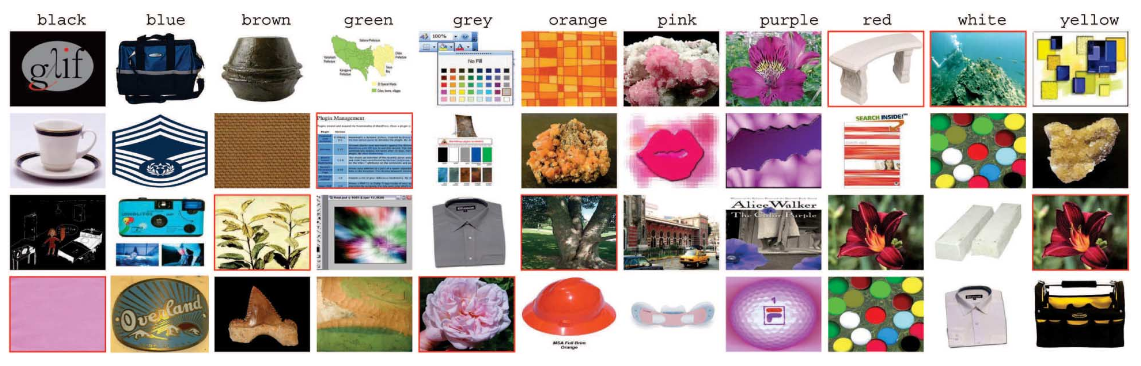
\includegraphics[width=1\textwidth]{image/lit/van20091.PNG}
\caption[Google-retrieved examples for colour names. The red bounding boxes indicate false positives. An image can be retrieved with various colour names, such as the flower image which appears in the red and the yellow set.]{Google-retrieved examples for colour names. The red bounding boxes indicate false positives. An image can be retrieved with various colour names, such as the flower image which appears in the red and the yellow set.  Reproduced from \citeA{van2009learning}.}
\label{fig:van20091}
\end{figure}

The PLSA model allows multiple colour terms to be named for each image. The pixels in the image (document) was discretized (quantized) into a finite vocabulary set of $10 \times 20 \times 20$ cubes of L*a*b colour space. Then, the image was represented using a histogram which indicates how many pixels are assigned to each bin (word). Now, given a set of documents $D = \{d_1, d_2, ... , d_N\}$ each described in a vocabulary $W = \{w_1, w_2, ... , w_M\}$, the words are taken to be generated by latent topics $Z = \{z_1, z_2, ... , z_K\}$. In the PLSA model the conditional probability of a word $w$ in a document $d$ is given by:
\begin{align}
    p(w|d) = \sum_{z\in Z}{p(w|z)p(z|d)}
\end{align}
The aim of $p(w|d)$ is to find latent topics which best explains the observed data, and in this case, finding the colour terms that best describes an image. In their approach, the authors claim that it their proposed method is flexible when new colour terms are introduced to any given system as the model can be trained with a small amount of data as compared to traditional methods which relies on chip based studies. 

\begin{figure}[hbt!]\centering
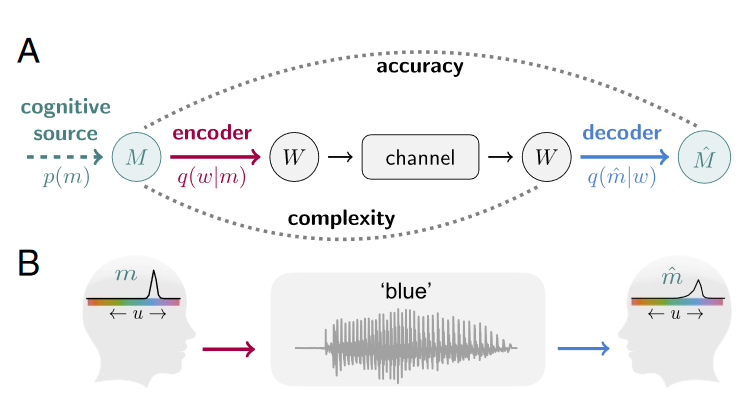
\includegraphics[width=1\textwidth]{image/lit/datacompress1.PNG}
\caption[(A) Shannon's communication model. In this model, the source message $M$ and its reconstruction $\hat{M}$ are distributions over objects in the universe $U$. We refer to these messages as meanings. $M$ is compressed into a code, or word, W. We assume that $W$ is transmitted over an idealised noiseless channel and that the reconstruction $\hat{M}$ of the source message is based on $W$. The accuracy of communication is determined by comparing $M$ and $\hat{M}$, and the complexity of the lexicon is determined by the mapping from $M$ to $W$. 
(B) Colour Communication Example,  where $U$ is a set of colours, shown for simplicity along a single dimension. A specific meaning $m$ is drawn from $p(m)$. The speaker communicates $m$ by uttering the word “blue”, and the listener interprets blue as meaning $\hat{m}$.
]
{(A) \citeA{shannon1948mathematical}'s communication model. In this model, the source message $M$ and its reconstruction $\hat{M}$ are distributions over objects in the universe $U$. We refer to these messages as meanings. $M$ is compressed into a code, or word, W. We assume that $W$ is transmitted over an idealised noiseless channel and that the reconstruction $\hat{M}$ of the source message is based on $W$. The accuracy of communication is determined by comparing $M$ and $\hat{M}$, and the complexity of the lexicon is determined by the mapping from $M$ to $W$. 
(B) Colour Communication Example,  where $U$ is a set of colours, shown for simplicity along a single dimension. A specific meaning $m$ is drawn from $p(m)$. The speaker communicates $m$ by uttering the word “blue”, and the listener interprets blue as meaning $\hat{m}$.
Reproduced from \citeA{zaslavsky2018efficient}.}
\label{fig:datacompression1}
\end{figure}

In the work of \cite{zaslavsky2018efficient}, the authors aimed to study efficient compression in colour naming and its evolution. \citeA{zaslavsky2018efficient} claims that colour categories cannot be hard-partitioned in the colour space, instead, a soft-partitioned approach should be taken. However, with a soft-partition approach, there are transition regions in the colour space that are often inconsistently named. 
In their work, the approached this challenge of understanding how colours are named from the angle of data compression. Figure \ref{fig:datacompression1} illustrates the idea of \citeA{zaslavsky2018efficient}'s work. The goal of this work is to design a Information Bottleneck (IB) compression model that represents can effectively represent colours terms in different languages. 

\citeA{yu2018beyond} proposed that the 11 common colour terms that are commonly use is insufficient. The work of \citeA{khan2013discriminative} agrees and suggests that colour representation that has been extended to more than the eleven dimensions could be beneficial. Instead, a dataset of 28 additional colour terms (a total of 39 terms) was used in their experiments on several task such as visual tracking, person re-identification as well as image classification. Similar to \citeA{van2009learning}'s work, \citeA{yu2018beyond} also applied PLSA to estimate the probability of colour values when given a colour term.






\begin{comment}
https://ieeexplore.ieee.org/stamp/stamp.jsp?tp=&arnumber=4982667&tag=1
https://www.pnas.org/content/pnas/115/31/7937.full.pdf
https://link.springer.com/content/pdf/10.1007%2Fs00138-017-0902-y.pdf
https://www.imbs.uci.edu/~kjameson/HinksCardenasKuehniEtAlJOSA2007.pdf
http://imbs.uci.edu/~kjameson/ECST/Kay_Cook_WorldColorSurvey.pdf
http://www.munsellcolourscienceforpainters.com/ConversionsBetweenMunsellAndsRGBsystems.pdf


\end{comment}



\cc{ the following statement needs to be removed}
Figure \ref{fig:munsell_ori330} shows the original Munsell 330 Colour chips which contains 10 achromatic colour chips and 320 chromatic colour chips. 
The 320 chromatic chips are 40 hues (at full saturation) which are evenly spaced out with 8 different levels of lightness (value) for each hue-value pair (\cite{kay2009world}).
These chips are also known as the World Colour Survey (WCS) stimulus palette.  
Figure \ref{fig:munsell_compare} shows the comparison of how the WCS stimulus palette were assigned colour terms using different methods; (a)Parametric model by \citeA{benavente2008parametric}; (b)  Probabilistic Latent Semantic Analysis (PLSA) - individual by \citeA{van2009learning}; (c) Linguistic and data compression approach by \citeA{zaslavsky2018efficient}; (d) The plot for our proposed method assigns the colour term that contains achieved the highest similarity score (\%) using Riemersma's low cost LUV estimation metrics.
The plot produced by our method shows similarity when compared with the plot produced using the linguistic approach. Comparing the parametric model (a) with the proposed method, it is noted that the achromatic tones were given more room to express its nature of low saturation value. However, as the assigning of colour terms are subjective to individuals, is it difficult to measure how well each method performed against each other. 


\subsubsection{Vehicle Motion Extraction}


\subsection{Object Semantics Retrieval}

According to the survey by \cite{chandran2017review}, trajectory retrieval algorithms can be largely divided into two categories: i) String  Matching Algorithm, and ii) Sketch Matching Algorithm. String matching algorithms   



\cc{include what type of semantics were extracted from which paper, take from proposal defense}

"For example, if themonitoring staves want to find a suspect vehicle in huge amount of surveillancevideos, they will firstly filter out large numbers of vehicles by appearance fea-tures, such as colors, shapes and types, to narrow down the search space."


longest   common   subsequence   (LCSS)   algorithm complete  string-based  matching  trajectories  by  per-forming  a  frame-by-frame  analysis  directly  on  ob-jects’ coordinates. The  work  in  [3]  assumed a  query  by  example  me-chanism  according  to  presented  example  trajectory and  the  search  system  could  return  a  ranked  list  of most similar items in the data set by a string matching algorithm,  whereas  the  sketch-based  method  projects a trajectory on a  set of basic functions and matches it according to its low-level geometrical features.